\documentclass[12pt, a4paper]{article}

\usepackage[a4paper, margin=2.5cm]{geometry}
\usepackage{fontspec}
\setmainfont{Liberation Serif}
\usepackage[portuguese, bidi=basic, provide=*]{babel}
\babelprovide[import, onchar=ids fonts]{portuguese}
\babelprovide[import, onchar=ids fonts]{english}

\usepackage{enumitem}
\setlist[itemize]{label=-}
\usepackage{amsmath}
\usepackage{booktabs}
\usepackage{tabularx}
\usepackage{array}
\usepackage{float}
\usepackage{graphicx}
\usepackage{caption}
\usepackage[table]{xcolor}
\usepackage{hyperref}

\definecolor{spaceblue}{RGB}{24, 43, 73}

\captionsetup{font=small, labelfont=bf}
\setlength{\fboxsep}{1pt}
\setlength{\fboxrule}{0.5pt}

\hypersetup{
    colorlinks=true,
    linkcolor=spaceblue,
    urlcolor=blue,
    pdftitle={Nabuus - Especificação, Arquitetura e Modelagem de Sistema},
    pdfauthor={Grupo Nabuus}
}

\setlength{\parskip}{0.5em}
\setlength{\parindent}{0pt}

\begin{document}

% -------------------------------------------------------------------
% CAPA
% -------------------------------------------------------------------
\begin{titlepage}
    \centering
    \vspace*{2.2cm}

    {\large \textsc{Universidade Federal de Juiz de Fora}}\\[0.2cm]
    {\normalsize \textsc{Trabalho Prático de Modelagem de Sistemas}}\\[2.6cm]

    \rule{\textwidth}{1.5pt}\\[0.6cm]
    {\Huge \textbf{\textcolor{spaceblue}{NABUUS}}}\\[0.3cm]
    {\Large \textit{Como seria viajar pelas estrelas?}}\\[0.4cm]
    \rule{\textwidth}{1.5pt}\\[1.8cm]

    {\LARGE \textbf{Documento de Arquitetura, Requisitos e Modelagem}}\\[1.4cm]

    \begin{flushright}
        \large
        \textbf{Equipe:}\\
        Davi Monção Fernandes\\
        David Élder Rodrigues Fraga\\
        Gabriel Andrioli Fonseca\\
        Gabriel Parreira Ferreira\\
        Pedro Miana Amaral
    \end{flushright}
    \vspace{1cm}

    \begin{tabular}{p{4.5cm}p{7cm}}
        \toprule
        \textbf{Entregável:} & Especificação Técnica, Processo e Modelagem UML/C4 \\
        \textbf{Data:} & Novembro de 2026 \\
        \bottomrule
    \end{tabular}

    \vfill

    {\small Juiz de Fora --- MG \\ 2026}
\end{titlepage}

% -------------------------------------------------------------------
% SUMÁRIO E LISTA DE FIGURAS
% -------------------------------------------------------------------
\pagenumbering{arabic}
\setcounter{page}{1}

\tableofcontents
\clearpage
\listoffigures
\newpage

% -------------------------------------------------------------------
% 1. CONTEXTUALIZAÇÃO, PROPÓSITO E ESCOPO DO PROJETO
% -------------------------------------------------------------------
\section{Contextualização, Propósito e Escopo do Projeto}

\subsection{Nome, Propósito e Conceito do Nabuus}
O projeto \textbf{Nabuus} nasce de uma especulação científica e criativa: \textit{``Como seria viajar pelas estrelas?''}. Seu propósito é permitir que usuários compreendam, de maneira interativa e intuitiva, as escalas reais de tempo, distância e custo envolvidas em viagens espaciais interestelares e intergalácticas. Para tornar essas grandezas palpáveis, o sistema traduz a experiência de navegação espacial para o fluxo cotidiano de compra de passagens rodoviárias inspirado na plataforma \textbf{ClickBus}.

A malha espacial é alimentada a partir de um catálogo astronômico real (\texttt{data/nabuus\_planetas.csv}), inicializado no banco com 36 sistemas estelares, 50 planetas (sendo 49 destinos distintos a partir da Terra), 12 ônibus espaciais com múltiplas versões de propulsão e capacidades padronizadas (\texttt{24}, \texttt{32} ou \texttt{48} poltronas), 17 rotas lúmicas e 196 viagens pré-carregadas via migrações Flyway (\texttt{V1} a \texttt{V3}).

A coordenação da plataforma divide-se em três perfis humanos e um subsistema científico:
\begin{itemize}
    \item \textbf{Astrônomo:} Mapeia a base técnica e científica da galáxia — cadastra sistemas solares, planetas (com indicação de posto de recarga), rotas lúmicas partindo do Sistema Solar, tecnologias de propulsão (com faixas de velocidade) e a frota técnica de ônibus espaciais.
    \item \textbf{Fretista:} Opera comercialmente as rotas — seleciona destino, ônibus espacial cadastrado e data de partida, utiliza o cálculo de preço sugerido ajustado à distância e à propulsão da nave, gerencia disponibilidade e publica viagens. Todos os cálculos físicos da linha são executados uma única vez no momento da publicação e persistidos em banco.
    \item \textbf{Usuário (Passageiro):} Pesquisa viagens publicadas ordenando por data mais próxima ou localidade mais próxima, escolhe propulsão disponível na nave, classe de cabine (\texttt{Executiva}, \texttt{Primeira classe} ou \texttt{Luxo} com criogenia), plano de alimentação (\texttt{Padrão}, \texttt{Vegetariana} ou \texttt{Gourmet}), compara os cenários \textbf{Com Rota Lúmica} e \textbf{Sem Rota Lúmica}, analisa o \textbf{Mapa Galáctico 2D} e seleciona sua poltrona no mapa da cabine para emitir o comprovante.
\end{itemize}

\subsection{Escopo, Limites do Sistema e Premissas Físicas}
O escopo do Nabuus abrange exclusivamente a simulação educacional e exploratória de viagens só de ida com origem no \textbf{Sistema Solar} (planeta Terra). O sistema adota premissas bem delimitadas:
\begin{itemize}
    \item \textbf{Cinemática Relativística Simplificada:} Cada trecho é modelado por aceleração própria constante ($g$), fase de cruzeiro em fração da velocidade da luz ($c$) e frenagem simétrica até o destino, portal lúmico ou posto de recarga, mantendo coerência nas ordens de grandeza sem integração orbital de $N$-corpos.
    \item \textbf{Posições Estacionárias Fixas:} As distâncias entre estrelas usam coordenadas equatoriais (RA, Dec) e distância ao Sol em anos-luz; dentro de cada sistema, considera-se distância radial fixa em Unidades Astronômicas (UA).
    \item \textbf{Pagamentos e Operação Simulados:} Não há integração com gateways financeiros reais ou sistemas externos de terceiros; a emissão do bilhete e o processamento de pagamento ocorrem integralmente de forma simulada no próprio sistema.
    \item \textbf{Caráter Didático das Escalas:} Os custos em créditos e as dívidas temporais atingem valores elevados propositalmente, evidenciando que, mesmo sob hipóteses futurísticas como propulsão por antimatéria ou rotas lúmicas, deslocamentos interestelares impõem severas barreiras econômicas e relativísticas.
\end{itemize}

\subsection{Glossário de Domínio}
\begin{table}[H]
\centering
\renewcommand{\arraystretch}{1.25}
\begin{tabularx}{\textwidth}{>{\bfseries}l X}
\toprule
Conceito & Descrição no Contexto do Nabuus \\
\midrule
Dívida Temporal & Tempo decorrido nos referenciais estacionários (Terra/destino) que excede o tempo vivido a bordo pelo passageiro, decorrente da dilatação temporal relativística. \\
Rota Lúmica & Canal hiperlúmico partindo do Sistema Solar rumo a outro sistema estelar. Dispensa paradas de recarga, porém impõe pedágio elevado e alta dívida temporal devido à fração extrema de $c$. \\
Tipo de Propulsão & Tecnologia científica cadastrada pelo astrônomo (ex.: Antimatéria, Fusão nuclear, Vela solar), especificando aceleração ($g$), faixa de velocidades ($c$), autonomia em anos-luz e tarifas de referência. \\
Ônibus Espacial & Aeronave interestelar registrada tecnicamente com capacidade fixa de \texttt{24}, \texttt{32} ou \texttt{48} poltronas e uma ou mais versões de propulsão suportadas. \\
Criogenia (Classe Luxo) & Recurso exclusivo da classe \texttt{Luxo} que desconta \texttt{90\%} do tempo desperto a bordo (\(\tau_{\text{desperto}} = 0{,}1\,\tau\)), mantendo a duração física total no referencial externo. \\
Planos de Alimentação & Serviços opcionais selecionados no checkout com acréscimos sobre a tarifa da classe: \texttt{Padrão} (+2\%), \texttt{Vegetariana} (+3\%) e \texttt{Gourmet} (+5\%). \\
Ocupação por Conforto & Distribuição determinística de assentos inicialmente ocupados gerada na publicação da viagem segundo a tecnologia/conforto (linhas econômicas são mais lotadas; linhas tecnológicas/luxo são mais livres). \\
Referencial da Nave & Tempo próprio ($\tau$) medido pelos relógios de bordo durante aceleração, cruzeiro e frenagem. \\
\bottomrule
\end{tabularx}
\end{table}

% -------------------------------------------------------------------
% 2. VISÃO ARQUITETURAL, USUÁRIOS E SISTEMAS EXTERNOS
% -------------------------------------------------------------------
\section{Visão Arquitetural, Usuários e Sistemas Externos}

\subsection{Tipos de Usuários e Subsistema Científico}
A operação do Nabuus é estruturada em torno de três perfis de usuários autenticados (RNF-01) e um subsistema computacional dedicado, sem dependências de serviços externos de terceiros:
\begin{enumerate}
    \item \textbf{Astrônomo:} Responsável pela base cartográfica e tecnológica. Autentica-se com credencial científica homologada (\texttt{IAU-2100-*}) para cadastrar, editar e remover sistemas solares, planetas (com postos de recarga), rotas lúmicas, tipos de propulsão e ônibus espaciais (\texttt{24}, \texttt{32} ou \texttt{48} assentos).
    \item \textbf{Fretista:} Responsável pela malha comercial e logística. Autentica-se com CNPJ intergaláctico homologado para selecionar ônibus espaciais da frota, consultar o preço sugerido calculado para o destino e a nave, publicar novas viagens, editar linhas e gerenciar disponibilidade.
    \item \textbf{Usuário (Passageiro):} Consumidor final que se cadastra com CPF e data de nascimento válida, pesquisa viagens pré-calculadas, ordena por proximidade temporal ou espacial, escolhe propulsão, classe, alimentação e cenário (Com/Sem Rota Lúmica), explora o Mapa Galáctico 2D e adquire passagem selecionando poltrona livre na classe escolhida.
    \item \textbf{Motor de Cálculo Físico (Subsistema Interno):} Microsserviço autônomo em Python (\texttt{FastAPI}) invocado pelo servidor Java no momento da publicação e na consulta de tarifas sugeridas. Executa validação de autonomia com indexação espacial (\texttt{cKDTree}), seleção gulosa de paradas de recarga, cinemática relativística, geração da rota 2D e ocupação inicial de poltronas.
\end{enumerate}

\subsection{Arquitetura em Contêineres e Decisões Técnicas}
O sistema adota arquitetura \textbf{Cliente-Servidor desacoplada} organizada em quatro contêineres orquestrados via \texttt{docker-compose.yml}: Front-End Web (\texttt{Nginx} na porta \texttt{3000} com proxy reverso \texttt{/api}), API de Negócios (\texttt{Java 21 / Spring Boot 3.4} na porta \texttt{8080}), Motor de Cálculo Físico (\texttt{Python 3.11 / FastAPI} na porta \texttt{8001}) e Banco de Dados Relacional (\texttt{PostgreSQL 16} na porta \texttt{5432} com versionamento Flyway).

\begin{table}[H]
\centering
\renewcommand{\arraystretch}{1.25}
\begin{tabularx}{\textwidth}{l l X}
\toprule
\textbf{Camada / Contêiner} & \textbf{Tecnologia} & \textbf{Responsabilidade Principal} \\
\midrule
Interface (Front-End) & HTML5, CSS3, JS (ES6) & Busca estilo ClickBus, comparação Com/Sem Rota Lúmica, seleção de propulsão/classe/alimentação, mapa de cabine e Mapa Galáctico 2D, com estado reativo seguro sem \texttt{innerHTML}. \\
Núcleo de Negócios (Back-End) & Java 21, Spring Boot & Controle de acesso JWT por papéis (\texttt{Controller -> Service -> Repository -> Entity}), gestão de catálogos, validação de frota (\texttt{24/32/48}), publicação de viagens e venda de passagens. \\
Motor Científico & Python 3.11, FastAPI, SciPy & Microsserviço \textit{stateless} acionado na publicação para sugestão de preços, paradas de recarga (\texttt{cKDTree}), cinemática relativística, rota 2D e ocupação inicial. \\
Persistência & PostgreSQL 16, Flyway & Armazenamento relacional ACID de usuários, catálogo estelar, propulsões, rotas lúmicas, viagens pré-calculadas (JSONB + colunas numéricas) e passagens, populado via \texttt{V1}--\texttt{V3}. \\
\bottomrule
\end{tabularx}
\end{table}

\paragraph{Decisão Arquitetural: Por que não MVC Tradicional?}
Em vez de um monólito MVC renderizado no servidor (como JSP ou Thymeleaf), adotou-se separação estrita entre Front-End estático, API REST em Java e microsserviço científico em Python por três razões técnicas: (i) \textbf{natureza poliglota} para aproveitar o ecossistema científico maduro do Python (\texttt{SciPy}, cálculos relativísticos e grafos); (ii) \textbf{isolamento de falhas e desempenho}, evitando que simulações físicas pesadas bloqueiem as \textit{threads} transacionais de autenticação e compra do servidor Java; e (iii) \textbf{experiência dinâmica de UI}, permitindo atualizações fluidas de filtros, classes, poltronas e mapas via JSON sem recarregar a página.

% -------------------------------------------------------------------
% 3. ESPECIFICAÇÃO DE REQUISITOS DO SISTEMA
% -------------------------------------------------------------------
\section{Especificação de Requisitos do Sistema}

\subsection{Requisitos Funcionais (RF) e Escala de Prioridade}
Para orientar o sequenciamento das Sprints e a entrega de valor do sistema, todos os requisitos funcionais foram classificados segundo uma escala de três níveis de prioridade:

\begin{table}[H]
\centering
\renewcommand{\arraystretch}{1.25}
\begin{tabularx}{\textwidth}{>{\bfseries}l X}
\toprule
Nível de Prioridade & Critério de Classificação \\
\midrule
Essencial & Requisito indispensável para a operação mínima viável (MVP) do simulador e para os fluxos centrais de cadastro cartográfico, publicação com cálculo único, busca e compra de passagens. \\
Importante & Requisito que agrega governança de dados, flexibilidade operacional, comparação de cenários (Com/Sem Lúmica, propulsões, criogenia) e ordenação/filtragem avançada. \\
Desejável & Requisito voltado à visualização gráfica enriquecida, ergonomia do usuário, sugestões automatizadas e legibilidade didática das escalas espaciais. \\
\bottomrule
\end{tabularx}
\end{table}

\subsubsection{Agente: Astrônomo}
\begin{itemize}
    \item \textbf{RF-01 --- Cadastrar sistemas solares [Essencial]:} Permite registrar sistemas estelares informando nome, estrela principal, ascensão reta (RA entre $0^\circ$ e $360^\circ$), declinação (Dec entre $-90^\circ$ e $90^\circ$) e distância ao Sol em anos-luz.
    \item \textbf{RF-02 --- Cadastrar planetas e postos de recarga [Essencial]:} Permite vincular planetas a um sistema solar informando nome, raio, massa, zona habitável, distância fixa à estrela em UA e indicação de posto de recarga (\texttt{possuiPostoRecarga}).
    \item \textbf{RF-03 --- Definir rotas lúmicas [Importante]:} Permite estabelecer canais partindo do Sistema Solar rumo a outros sistemas, informando velocidade sub-relativística ($0 < v < 1\,c$), valor de pedágio e status \texttt{ativa}.
    \item \textbf{RF-04 --- Cadastrar tipos de propulsão [Essencial]:} Permite registrar tecnologias de propulsão definindo aceleração própria ($g$), faixa de velocidade mínima e máxima ($c \le 0{,}4$), autonomia em anos-luz e valores de referência.
    \item \textbf{RF-05 --- Editar e remover cadastros cartográficos [Importante]:} Permite atualizar ou desativar registros de malha e propulsão, suspendendo automaticamente (\texttt{status = SUSPENSA}) as viagens ativas vinculadas a rotas lúmicas desativadas.
    \item \textbf{RF-06 --- Cadastrar ônibus espaciais [Essencial]:} Permite ao astrônomo registrar veículos espaciais informando identificação única, capacidade padronizada de poltronas (\texttt{24}, \texttt{32} ou \texttt{48}) e uma ou mais versões de propulsão suportadas dentro das faixas técnicas cadastradas.
    \item \textbf{RF-10 --- Gerenciar frota técnica de naves [Importante]:} Permite consultar ou remover ônibus espaciais do catálogo técnico utilizado nas viagens.
\end{itemize}

\subsubsection{Agente: Fretista}
\begin{itemize}
    \item \textbf{RF-07 --- Criar, editar e publicar viagens [Essencial]:} Permite selecionar destino, ônibus espacial cadastrado pela equipe científica (herdando automaticamente sua capacidade de \texttt{24}, \texttt{32} ou \texttt{48} poltronas) e data futura válida (\texttt{dd/mm/aaaa}), acionando o motor físico para validar autonomia e persistir os cenários Com e Sem Rota Lúmica.
    \item \textbf{RF-08 --- Consultar preço sugerido e definir tarifa [Desejável]:} Permite visualizar a fórmula dinâmica calculada para o destino e a nave selecionados e aplicar com um clique o preço sugerido (\texttt{"Preço sugerido aplicado!"}), inicializando novas viagens com preço \texttt{0} para preenchimento explícito ou ajuste pelo fretista.
    \item \textbf{RF-09 --- Gerenciar disponibilidade de viagens [Importante]:} Permite listar, editar, publicar ou excluir/suspender viagens oferecidas sob responsabilidade operacional do fretista.
\end{itemize}

\subsubsection{Agente: Usuário (Passageiro)}
\begin{itemize}
    \item \textbf{RF-11 --- Buscar viagens por origem, destino e data [Essencial]:} Permite consultar as viagens publicadas entre a Terra e o sistema ou planeta de destino desejado com data de partida válida no futuro.
    \item \textbf{RF-12 --- Filtrar e ordenar resultados [Importante]:} Permite filtrar por tecnologias de propulsão e distância máxima (em anos-luz), além de ordenar por \textbf{Data mais próxima} ou \textbf{Localidade mais próxima}.
    \item \textbf{RF-13 --- Visualizar resumo e comparar cenários [Importante]:} Exibe nos cards de resultado as classes, propulsões suportadas e disponibilidade de Rota Lúmica; na tela da viagem, compara os cenários \textbf{Com Rota Lúmica} e \textbf{Sem Rota Lúmica}, além de permitir alternar propulsão, classe (com criogenia de \texttt{90\%} na \texttt{Luxo}) e alimentação (\texttt{2\%}, \texttt{3\%}, \texttt{5\%}).
    \item \textbf{RF-14 --- Selecionar poltrona por classe e comprar passagem [Essencial]:} Exibe o mapa dinâmico de \texttt{24}, \texttt{32} ou \texttt{48} assentos da nave, restringe a seleção à classe escolhida, alerta caso haja divergência de classe e emite o comprovante de passagem.
    \item \textbf{RF-15 --- Visualizar rota no Mapa Galáctico 2D [Desejável]:} Apresenta graficamente em 2D o trajeto pré-calculado da viagem, destacando origem, paradas de reabastecimento, destino e eventual trânsito lúmico.
\end{itemize}

\subsubsection{Subsistema: Módulos de Cálculo Físico}
\begin{itemize}
    \item \textbf{RF-16 --- Sugerir tarifação por propulsão e distância [Desejável]:} Calcula o preço base, custo por ano-luz e paradas estimadas com base no tipo de propulsão, conforto e distância real ao planeta de destino.
    \item \textbf{RF-17 --- Calcular duração no referencial da nave [Essencial]:} Determina o tempo próprio vivido a bordo ($\Delta t_{\text{bordo}}$) integrando etapas de aceleração constante, cruzeiro e frenagem simétrica em cada salto (e trânsito lúmico quando aplicável).
    \item \textbf{RF-18 --- Calcular dívida temporal [Importante]:} Estima a diferença entre o tempo decorrido nos referenciais estacionários e o tempo próprio da nave:
    \begin{equation}
        D_{\text{temporal}} = \Delta t_{\text{estacionário}} - \Delta t_{\text{bordo}}
    \end{equation}
    \item \textbf{RF-19 --- Validar autonomia e paradas pela regra gulosa [Essencial]:} Verifica o alcance da nave frente à distância do trajeto e seleciona sucessivamente o posto de recarga alcançável mais avançado rumo ao destino, gerando os trechos da rota 2D.
    \item \textbf{RF-20 --- Calcular preços finais dos cenários [Essencial]:} Determina os preços finais somando preço base, custo por ano-luz multiplicado pela distância, custo por parada de recarga e pedágio lúmico (além de multiplicadores de classe e alimentação no checkout).
    \item \textbf{RF-21 --- Gerar ocupação inicial de assentos [Importante]:} Seleciona deterministicamente (semente = \texttt{viagemId}) os assentos inicialmente ocupados em função da categoria de conforto (\texttt{ECONOMICA} mais lotada; \texttt{LUXO} mais vazia).
    \item \textbf{RF-22 --- Converter escalas de distância e tempo [Desejável]:} Transforma grandezas astronômicas e temporais extensas em notação legível para o público geral (UA, anos-luz, meses, anos, milhares ou bilhões).
\end{itemize}

\subsection{Requisitos Não-Funcionais (RNF)}
\begin{table}[H]
\centering
\renewcommand{\arraystretch}{1.25}
\begin{tabularx}{\textwidth}{l l X}
\toprule
\textbf{Código} & \textbf{Categoria} & \textbf{Especificação do Requisito} \\
\midrule
RNF-01 & Segurança & Autenticação stateless via JWT, senhas com BCrypt, validação de credenciais/CNPJs homologados, prevenção contra XSS no front-end sem uso de \texttt{innerHTML} e controle de acesso por papel. \\
RNF-02 & Modelagem & Cinemática relativística simplificada, porém fisicamente coerente nas ordens de grandeza e propagação de escalas. \\
RNF-03 & Arquitetura & Motor de cálculo físico \textit{stateless}, isolado em contêiner próprio e desacoplado da persistência transacional. \\
RNF-04 & Desempenho & Simulação completa na publicação em até 3 segundos; buscas e filtros dos passageiros leem dados pré-calculados diretamente no PostgreSQL. \\
RNF-05 & Usabilidade & Fluxo de busca, comparação de cenários e escolha de poltrona inspirado no padrão familiar do ClickBus. \\
RNF-06 & Usabilidade & Apresentação leve de métricas relativísticas, criogenia e rotas espaciais no Mapa Galáctico 2D. \\
RNF-07 & Interface & Interface Web responsiva com Design Tokens unificados (\texttt{tokens.css}), suportando desktop e dispositivos móveis. \\
RNF-08 & Escalabilidade & Catálogo espacial extensível com indexação \texttt{cKDTree} no motor Python e versionamento de dados em PostgreSQL via Flyway (\texttt{V1}--\texttt{V3}). \\
RNF-09 & Manutenibilidade & Arquitetura modular em camadas no Java, ES Modules no front-end e execução unificada com \texttt{docker compose up --build}. \\
\bottomrule
\end{tabularx}
\end{table}

\clearpage
\subsection{Matriz de Prioridades, Dependências e Rastreabilidade}
\begin{table}[H]
\centering
\footnotesize
\setlength{\tabcolsep}{4pt}
\renewcommand{\arraystretch}{1.08}
\begin{tabularx}{\textwidth}{l >{\raggedright\arraybackslash}X l l l}
\toprule
\textbf{Código} & \textbf{Título do Requisito} & \textbf{Prioridade} & \textbf{Pré-requisitos} & \textbf{Caso de Uso} \\
\midrule
RF-01 & Cadastrar sistemas solares & Essencial & --- & UC-01 \\
RF-02 & Cadastrar planetas e postos de recarga & Essencial & RF-01 & UC-01 \\
RF-03 & Definir rotas lúmicas & Importante & RF-01 & UC-01 \\
RF-04 & Cadastrar tipos de propulsão & Essencial & --- & UC-01 \\
RF-05 & Editar/remover cadastros e suspender viagens & Importante & RF-01 a RF-04 & UC-01 \\
RF-06 & Cadastrar ônibus espaciais (24/32/48 assentos) & Essencial & RF-04 & UC-01 \\
RF-07 & Criar, editar e publicar viagens (cálculo único) & Essencial & RF-02, RF-06, RF-17 a RF-21 & UC-02 \\
RF-08 & Consultar preço sugerido e definir tarifa & Desejável & RF-04, RF-16 & UC-02 \\
RF-09 & Gerenciar disponibilidade de viagens & Importante & RF-07 & UC-02 \\
RF-10 & Gerenciar frota técnica de naves & Importante & RF-06 & UC-01 \\
RF-11 & Buscar viagens por origem, destino e data & Essencial & RF-07, RF-09 & UC-03 \\
RF-12 & Filtrar e ordenar resultados (data/localidade) & Importante & RF-11 & UC-03 \\
RF-13 & Comparar cenários Com/Sem Lúmica e opções & Importante & RF-11, RF-22 & UC-03 \\
RF-14 & Selecionar poltrona por classe e comprar passagem & Essencial & RF-13, RF-21 & UC-04 \\
RF-15 & Visualizar rota no Mapa Galáctico 2D & Desejável & RF-11, RF-19 & UC-03 \\
RF-16 & Sugerir tarifação por propulsão e distância & Desejável & RF-04 & UC-02 \\
RF-17 & Calcular duração no referencial da nave & Essencial & RF-01, RF-02, RF-04 & UC-02 \\
RF-18 & Calcular dívida temporal relativística & Importante & RF-17 & UC-02 \\
RF-19 & Validar autonomia e paradas (regra gulosa) & Essencial & RF-02, RF-04 & UC-02 \\
RF-20 & Calcular preços finais dos cenários & Essencial & RF-03, RF-08, RF-19 & UC-02 \\
RF-21 & Gerar ocupação inicial de assentos & Importante & RF-06, RF-07 & UC-02 \\
RF-22 & Converter escalas de distância e tempo & Desejável & RF-17, RF-18 & UC-02, UC-03 \\
\bottomrule
\end{tabularx}
\end{table}

% -------------------------------------------------------------------
% 4. DIRETRIZES DE DOMÍNIO E CASOS DE USO
% -------------------------------------------------------------------
\section{Diretrizes de Domínio e Especificação de Casos de Uso}

\subsection{Diretrizes e Invariantes de Modelagem}
\begin{enumerate}
    \item \textbf{Dinâmica de Propulsão e Paradas:} Cada salto entre paradas divide-se em aceleração própria constante, cruzeiro e frenagem simétrica, considerando desprezível o tempo estacionário de reabastecimento frente à duração interestelar.
    \item \textbf{Dois Cenários por Viagem:} Sem rota lúmica, o deslocamento ocorre diretamente entre planetas (com eventuais escalas em postos de recarga). Com rota lúmica, o trajeto percorre a distância em UA até a estrela de origem, cruza o canal lúmico e finaliza em UA até o planeta de destino.
    \item \textbf{Capacidade Padronizada Vinculada à Nave:} Cada ônibus espacial possui exatamente \texttt{24}, \texttt{32} ou \texttt{48} poltronas distribuídas em zonas de \texttt{Luxo}, \texttt{Primeira classe} e \texttt{Executiva}. O fretista não define manualmente a lotação da viagem; esta herda automaticamente a capacidade da nave escolhida.
    \item \textbf{Criogenia, Classes e Alimentação:} A classe \texttt{Luxo} inclui criogenia com desconto de \texttt{90\%} sobre o tempo desperto a bordo e fator tarifário \texttt{2x} (\texttt{Primeira classe} aplica \texttt{1,5x}; \texttt{Executiva} aplica \texttt{1x}). Planos de alimentação somam \texttt{2\%}, \texttt{3\%} ou \texttt{5\%} conforme a escolha do viajante.
    \item \textbf{Cálculo Único na Publicação:} Duração a bordo, dívida temporal, preços finais, paradas/rota 2D e ocupação inicial são calculados na publicação da viagem e persistidos no banco, garantindo consultas instantâneas ao passageiro.
\end{enumerate}

\subsection{Especificação de Casos de Uso (UC)}

\subsubsection{UC-01 --- Gerenciar Malha Cartográfica, Propulsões e Naves}
\begin{itemize}
    \item \textbf{Ator:} Astrônomo.
    \item \textbf{Resumo:} O astrônomo autenticado registra sistemas solares (RF-01), planetas e postos de recarga (RF-02), rotas lúmicas (RF-03), tecnologias de propulsão com faixas de velocidade (RF-04) e ônibus espaciais com \texttt{24}, \texttt{32} ou \texttt{48} assentos e múltiplas versões de propulsão (RF-06, RF-10). Ao desativar rotas em uso, o sistema suspende automaticamente as viagens vinculadas (RF-05).
\end{itemize}

\subsubsection{UC-02 --- Operar Frota Comercial e Publicar Viagens Espaciais}
\begin{itemize}
    \item \textbf{Ator:} Fretista e Motor de Cálculo Físico.
    \item \textbf{Resumo:} O fretista seleciona destino, ônibus espacial cadastrado e data futura (RF-07), consulta a sugestão tarifária dinâmica recalculada pela fórmula e distância do planeta (RF-08, RF-16) e publica a viagem. O motor físico valida autonomia e define paradas gulosas e rota 2D (RF-19), calcula duração a bordo, dívida temporal, preços e escalas textuais (RF-17, RF-18, RF-20, RF-22) e gera a ocupação inicial (RF-21). O fretista também edita ou suspende suas linhas publicadas (RF-09).
\end{itemize}

\subsubsection{UC-03 --- Consultar Viagens, Comparar Cenários e Mapa 2D}
\begin{itemize}
    \item \textbf{Ator:} Usuário (Passageiro).
    \item \textbf{Resumo:} O passageiro pesquisa trajetos persistidos no banco (RF-11), filtra por propulsão ou distância e ordena por \textit{Data mais próxima} ou \textit{Localidade mais próxima} (RF-12), compara cenários Com e Sem Rota Lúmica com troca de propulsão, classe e alimentação (RF-13) e visualiza o trajeto no Mapa Galáctico 2D (RF-15).
\end{itemize}

\subsubsection{UC-04 --- Escolher Poltrona por Classe e Comprar Passagem}
\begin{itemize}
    \item \textbf{Ator:} Usuário (Passageiro).
    \item \textbf{Resumo:} O passageiro visualiza o mapa de poltronas da nave (\texttt{24}, \texttt{32} ou \texttt{48} lugares), seleciona uma poltrona livre pertencente à classe previamente escolhida, confirma o pagamento simulado e obtém o comprovante de passagem (RF-14).
\end{itemize}

% -------------------------------------------------------------------
% 5. MODELO DE PROCESSO ADOTADO E GESTÃO DO PROJETO
% -------------------------------------------------------------------
\section{Modelo de Processo Adotado e Gestão do Projeto}

\subsection{Framework Ágil Adotado (Scrum Adaptado)}
Para conduzir a concepção, modelagem e implementação do Nabuus com baixo atrito burocrático e alta frequência de validação, a equipe adotou o modelo de processo \textbf{Scrum adaptado}, apoiado por gestão visual em quadro \textbf{Kanban} no Trello e fluxo de versionamento \textbf{GitHub Flow} com \textit{Conventional Commits}. A escolha pelo Scrum se justifica pela necessidade de iterar rapidamente sobre regras físicas, modelo de domínio e interface ClickBus mantendo entregas incrementais funcionais ao final de cada ciclo.

\subsection{Estrutura e Duração das Sprints}
O projeto foi estruturado em \textbf{4 Sprints consecutivas com duração fixa de 1 semana (7 dias) cada}, totalizando 4 semanas de execução. As reuniões de \textit{Sprint Planning} (definição do \textit{Sprint Backlog}) e \textit{Sprint Review} ocorreram regularmente às \textbf{segundas-feiras}:
\begin{enumerate}
    \item \textbf{Sprint 1 (Semana 1) --- Concepção, Processo e Levantamento:} Definição do nome, propósito e escopo do Nabuus, estabelecimento do fluxo ágil, levantamento dos Requisitos Não-Funcionais (\texttt{RNF-01} a \texttt{RNF-09}) e modelagem preliminar de Casos de Uso.
    \item \textbf{Sprint 2 (Semana 2) --- Modelagem UML, Arquitetura e DER:} Elaboração dos diagramas de Arquitetura C4 (Contexto e Contêineres), Diagrama de Classes, Diagramas de Atividades (\texttt{AD01}--\texttt{AD03}), Diagramas de Sequência (\texttt{SD1}--\texttt{SD4}), DER do PostgreSQL e especificação detalhada e priorizada dos \texttt{RF-01} a \texttt{RF-22}.
    \item \textbf{Sprint 3 (Semana 3) --- Catálogo Científico, Motor Python e Protótipo Figma:} Curadoria do catálogo astronômico real (\texttt{nabuus\_planetas.csv}), implementação dos algoritmos relativísticos e espaciais no microsserviço Python (\texttt{FastAPI/SciPy}) e concepção integral do protótipo de alta fidelidade no \textbf{Figma} (\texttt{context/Nabuus.fig}).
    \item \textbf{Sprint 4 (Semana 4) --- Back-End Java, Front-End Web, Integração Docker e Testes:} Implementação da API REST Spring Boot com JWT e migrações Flyway (\texttt{V1}--\texttt{V3}), desenvolvimento da interface Web estática em ES Modules, empacotamento em 4 contêineres Docker Compose, refinamentos de usabilidade (preço sugerido dinâmico, restrição 24/32/48 assentos, ordenação de busca) e execução das suítes de testes automatizados.
\end{enumerate}

\subsection{Papéis Scrum e Responsabilidades da Equipe}
Mantendo uma equipe de desenvolvimento multifuncional e colaborativa, foram atribuídos formalmente os papéis do Scrum aliados às frentes técnicas desempenhadas por cada um dos cinco integrantes:

\begin{table}[H]
\centering
\renewcommand{\arraystretch}{1.25}
\begin{tabularx}{\textwidth}{l l X}
\toprule
\textbf{Integrante} & \textbf{Papel Scrum} & \textbf{Responsabilidades Principais no Projeto} \\
\midrule
Gabriel Andrioli Fonseca & \textit{Product Owner (PO)} & Visão do produto, priorização do \textit{Product Backlog}, validação funcional do catálogo, fluxos de front-end, orquestração Docker Compose e testes. \\
Pedro Miana Amaral & \textit{Scrum Master (SM)} & Condução das reuniões semanais de Sprint e remoção de impedimentos; segurança JWT/Spring Security, regras de negócio do back-end, modelagem UML e suítes de testes. \\
Davi Monção Fernandes & \textit{Dev Team} & Regras e validações de autenticação e cadastro de usuários (\texttt{dd/mm/aaaa}, senha), ajustes de Docker Compose e integração. \\
David Élder Rodrigues Fraga & \textit{Dev Team} & Modelagem e implementação das regras de precificação por classe e planos de alimentação no domínio e na interface. \\
Gabriel Parreira Ferreira & \textit{Dev Team} & Fluxo de seleção de poltronas por classe, padronização de calendário de partida na busca e ajustes do painel do fretista. \\
\bottomrule
\end{tabularx}
\end{table}

\subsection{Artefatos de Gestão e Recursos Tecnológicos}
\begin{itemize}
    \item \textbf{Artefatos Scrum:} \textit{Product Backlog} (lista priorizada de RFs), \textit{Sprint Backlog} semanal no Trello e Incremento integrado ao repositório principal via \textit{Pull Requests} após validação de build e testes.
    \item \textbf{Ferramentas de Apoio:} \textbf{Trello} (quadro Kanban das Sprints), \textbf{GitHub} (controle de versão e rastreamento de entregas), \textbf{Figma} (prototipação UI/UX), \textbf{PlantUML} (diagramas versionados como código) e \textbf{LaTeX / XeLaTeX} (compilação reprodutível deste documento).
\end{itemize}

% -------------------------------------------------------------------
% 6. MODELAGEM UML E ARQUITETURAL DO SISTEMA
% -------------------------------------------------------------------
\clearpage
\section{Modelagem UML e Arquitetural do Sistema}

Esta seção apresenta os diagramas gerados a partir das especificações em PlantUML versionadas em \texttt{context/}, cobrindo requisitos funcionais, comportamento, estrutura de classes, modelo de dados, arquitetura C4 e interações em sequência.

\subsection{Diagrama de Casos de Uso}
A Figura~\ref{fig:casos-de-uso} consolida os quatro grandes pacotes de casos de uso (\texttt{UC1} a \texttt{UC4}), os atores envolvidos (\texttt{Astrônomo}, \texttt{Fretista}, \texttt{Passageiro} e o subsistema \texttt{Motor de Cálculo Físico}) e a rastreabilidade direta de todos os requisitos funcionais numerados (\texttt{RF-01} a \texttt{RF-22}).

\begin{figure}[H]
    \centering
    \includegraphics[width=\textwidth, height=0.62\textheight, keepaspectratio]{figuras/casos-de-uso.pdf}
    \caption{Diagrama Geral de Casos de Uso do Sistema Nabuus com códigos \texttt{RF-01} a \texttt{RF-22}.}
    \label{fig:casos-de-uso}
\end{figure}

\clearpage
\subsection{Diagramas de Atividades}
Os Diagramas de Atividades (\texttt{AD01}, \texttt{AD02} e \texttt{AD03}), ilustrados nas Figuras~\ref{fig:ad01} a~\ref{fig:ad03}, detalham o fluxo de controle e as decisões nos cenários de busca/compra de passagem, gestão da malha cartográfica e publicação de linhas com cálculo único.

\begin{figure}[H]
    \centering
    \includegraphics[width=0.90\textwidth, height=0.66\textheight, keepaspectratio]{figuras/ad01-comprar-passagem.pdf}
    \caption{Diagrama de Atividades AD01 --- Pesquisar Viagem e Comprar Passagem Intergaláctica.}
    \label{fig:ad01}
\end{figure}

\begin{figure}[H]
    \centering
    \includegraphics[width=0.90\textwidth, height=0.72\textheight, keepaspectratio]{figuras/ad02-gerenciar-malha.pdf}
    \caption{Diagrama de Atividades AD02 --- Gerenciar Malha Cartográfica e Propulsões.}
    \label{fig:ad02}
\end{figure}

\begin{figure}[H]
    \centering
    \includegraphics[width=0.90\textwidth, height=0.76\textheight, keepaspectratio]{figuras/ad03-publicar-linha.pdf}
    \caption{Diagrama de Atividades AD03 --- Publicar Viagem Espacial com Cálculo Único.}
    \label{fig:ad03}
\end{figure}

\clearpage
\subsection{Diagrama de Classes}
A Figura~\ref{fig:diagrama-classes} apresenta as entidades de domínio, enums, hierarquia de usuários e os contratos de DTOs utilizados na comunicação com o \texttt{MotorCalculoClient}.

\begin{figure}[H]
    \centering
    \includegraphics[width=\textwidth, height=0.72\textheight, keepaspectratio]{figuras/diagrama-classes.pdf}
    \caption{Diagrama de Classes UML --- Entidades de Domínio, Enums e Contratos de Integração.}
    \label{fig:diagrama-classes}
\end{figure}

\clearpage
\subsection{Modelo Entidade-Relacionamento (DER PostgreSQL)}
A Figura~\ref{fig:diagrama-er} complementa a visão estrutural exibindo o esquema relacional implementado nas migrações do PostgreSQL (\texttt{V1}--\texttt{V3}), incluindo herança \textit{JOINED} de usuários, restrições de integridade e colunas \texttt{JSONB} (\texttt{rota\_2d\_json} e \texttt{assentos\_ocupados\_json}).

\begin{figure}[H]
    \centering
    \includegraphics[width=\textwidth, height=0.70\textheight, keepaspectratio]{figuras/diagrama-er.pdf}
    \caption{Diagrama Entidade-Relacionamento (DER / Modelo Físico PostgreSQL) do Sistema Nabuus.}
    \label{fig:diagrama-er}
\end{figure}

\clearpage
\subsection{Arquitetura em Modelo C4 (Contexto e Contêineres)}
As Figuras~\ref{fig:c4-contexto} e~\ref{fig:c4-conteineres} ilustram a arquitetura sob o Modelo C4 nos níveis 1 (Contexto) e 2 (Contêineres), evidenciando a comunicação entre Front-End, API Spring Boot, Banco PostgreSQL e Motor de Cálculo Físico em Python.

\begin{figure}[H]
    \centering
    \includegraphics[width=\textwidth, height=0.58\textheight, keepaspectratio]{figuras/c4-contexto.png}
    \caption{Modelo C4 (Nível 1) --- Diagrama de Contexto do Sistema Nabuus.}
    \label{fig:c4-contexto}
\end{figure}

\begin{figure}[H]
    \centering
    \includegraphics[width=\textwidth, height=0.68\textheight, keepaspectratio]{figuras/c4-conteineres.png}
    \caption{Modelo C4 (Nível 2) --- Diagrama de Contêineres e Protocolos de Comunicação.}
    \label{fig:c4-conteineres}
\end{figure}

\clearpage
\subsection{Diagramas de Sequência}
As Figuras~\ref{fig:sd1} a~\ref{fig:sd4} detalham a troca temporal de mensagens entre Interface Web, Controllers REST, Services, Repositories/PostgreSQL e o Motor Físico em Python.

\begin{figure}[H]
    \centering
    \includegraphics[width=\textwidth, height=0.68\textheight, keepaspectratio]{figuras/sd1-gerenciar-malha.pdf}
    \caption{Diagrama de Sequência SD1 --- Gerenciar Malha Cartográfica e Propulsões.}
    \label{fig:sd1}
\end{figure}

\begin{figure}[H]
    \centering
    \includegraphics[width=\textwidth, height=0.76\textheight, keepaspectratio]{figuras/sd2-publicar-viagem.pdf}
    \caption{Diagrama de Sequência SD2 --- Operar Frota e Publicar Viagem Espacial.}
    \label{fig:sd2}
\end{figure}

\begin{figure}[H]
    \centering
    \includegraphics[width=\textwidth, height=0.74\textheight, keepaspectratio]{figuras/sd3-consultar-viagens.pdf}
    \caption{Diagrama de Sequência SD3 --- Consultar Viagens, Comparar Cenários e Mapa 2D.}
    \label{fig:sd3}
\end{figure}

\begin{figure}[H]
    \centering
    \includegraphics[width=\textwidth, height=0.74\textheight, keepaspectratio]{figuras/sd4-comprar-passagem.pdf}
    \caption{Diagrama de Sequência SD4 --- Escolher Modalidade, Assento e Comprar Passagem.}
    \label{fig:sd4}
\end{figure}

% -------------------------------------------------------------------
% 7. PROTÓTIPO DE INTERFACE E MOCKUPS
% -------------------------------------------------------------------
\clearpage
\section{Protótipo de Interface e Mockups}

O design visual do Nabuus foi concebido previamente no \textbf{Figma}, com o arquivo-fonte versionado no próprio repositório em \texttt{context/Nabuus.fig}. A partir desse protótipo foram extraídos os \textit{Design Tokens} globais (\texttt{frontend/css/tokens.css}), consolidando a identidade escura estelar, a tipografia \texttt{Michroma}, os componentes BEM e a jornada de compra estilo ClickBus.

\begin{quote}
\textbf{Artefato de Prototipação:} Arquivo \texttt{context/Nabuus.fig} no repositório oficial do projeto. Caso seja disponibilizada uma URL pública de compartilhamento no Figma para visualização web, ela pode ser referenciada diretamente neste bloco antes da submissão final.
\end{quote}

As Figuras~\ref{fig:tela-home} a~\ref{fig:tela-astronomo} apresentam as principais telas da aplicação implementadas fielmente a partir dos mockups definidos no protótipo.

\begin{figure}[H]
    \centering
    \fbox{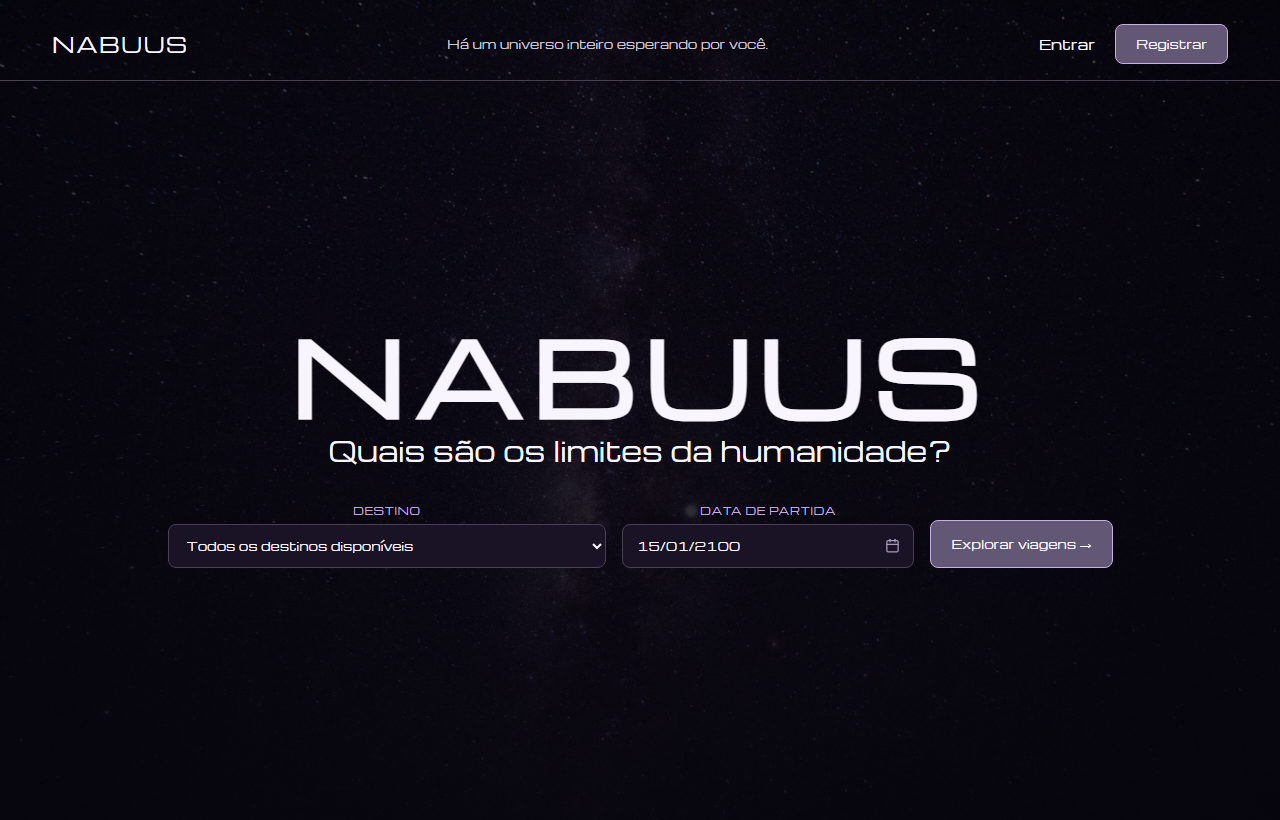
\includegraphics[width=0.78\textwidth, keepaspectratio]{figuras/tela-home.jpg}}
    \caption{Tela Inicial --- Busca interestelar com seleção de destino e data em calendário.}
    \label{fig:tela-home}
\end{figure}

\begin{figure}[H]
    \centering
    \fbox{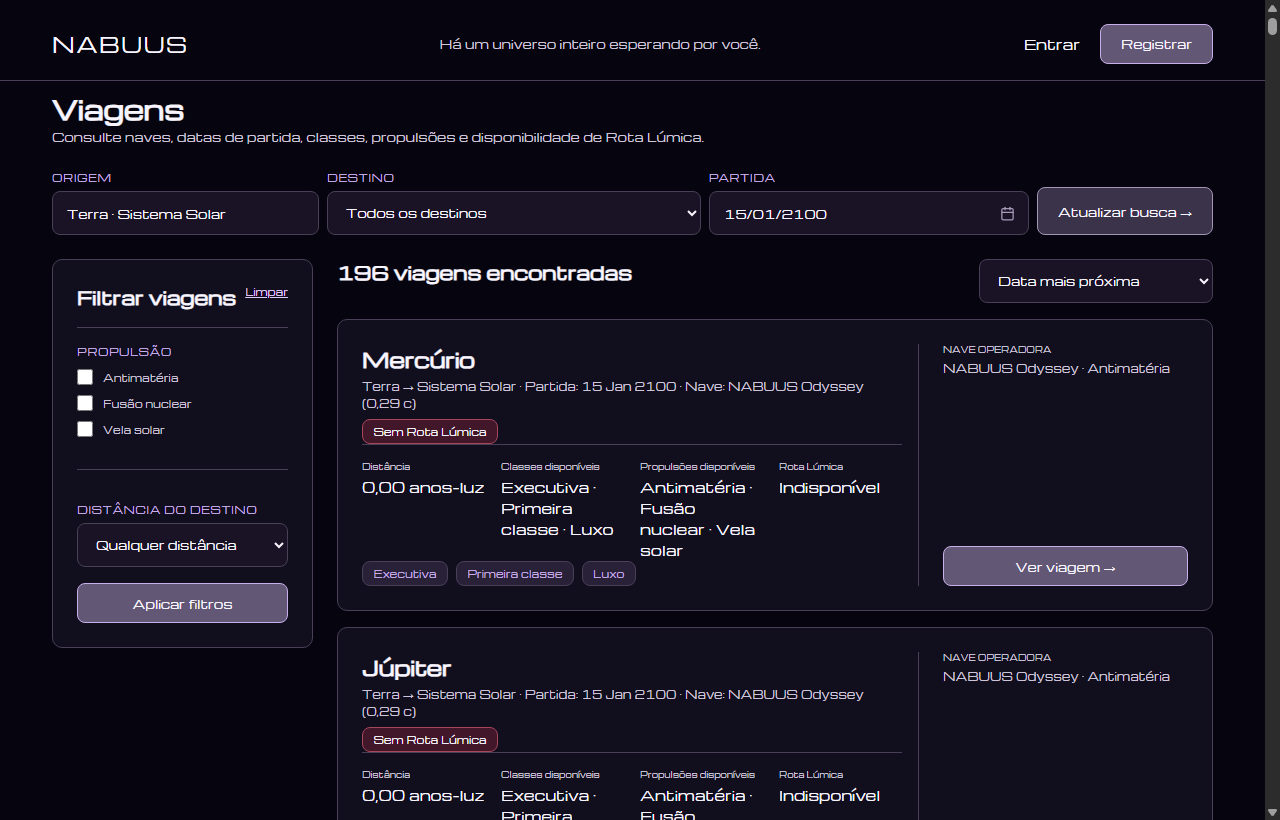
\includegraphics[width=0.86\textwidth, keepaspectratio]{figuras/tela-resultados.jpg}}
    \caption{Resultados da Busca --- Filtros por propulsão/distância e ordenação por data ou localidade mais próxima.}
    \label{fig:tela-resultados}
\end{figure}

\begin{figure}[H]
    \centering
    \fbox{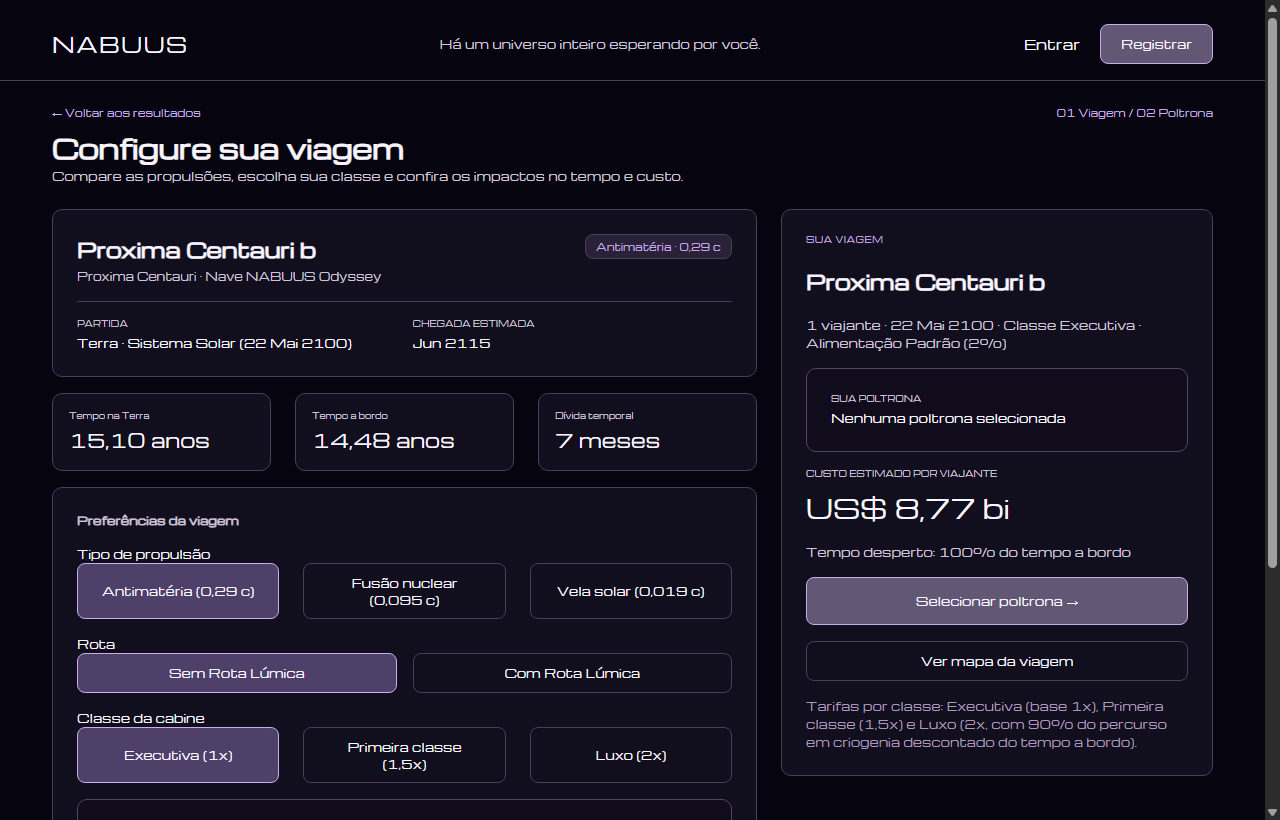
\includegraphics[width=0.86\textwidth, keepaspectratio]{figuras/tela-detalhes.jpg}}
    \caption{Detalhes da Viagem --- Comparação de propulsões, classes (criogenia), alimentação e Rota Lúmica.}
    \label{fig:tela-detalhes}
\end{figure}

\begin{figure}[H]
    \centering
    \fbox{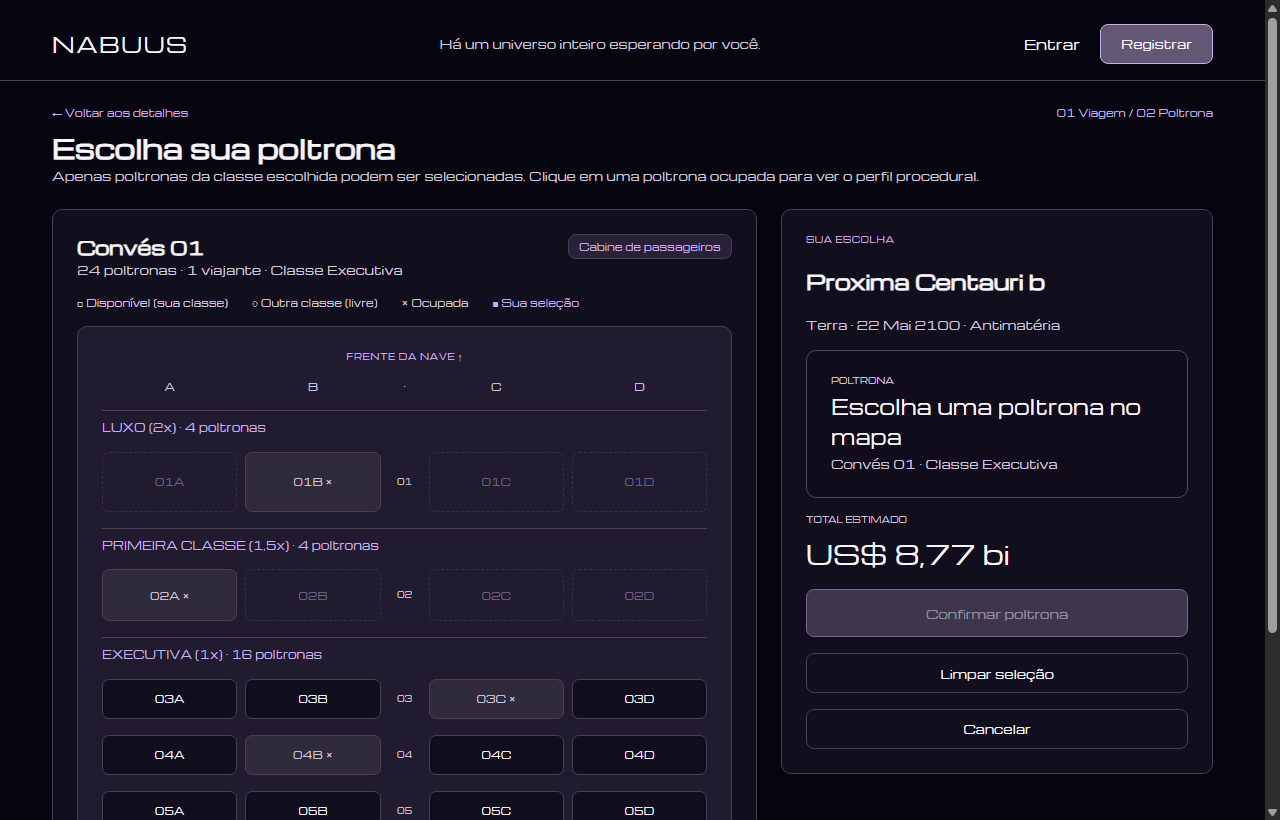
\includegraphics[width=0.86\textwidth, keepaspectratio]{figuras/tela-poltronas.jpg}}
    \caption{Seleção de Poltrona --- Mapa dinâmico da cabine com destaque visual por classe e ocupação.}
    \label{fig:tela-poltronas}
\end{figure}

\begin{figure}[H]
    \centering
    \fbox{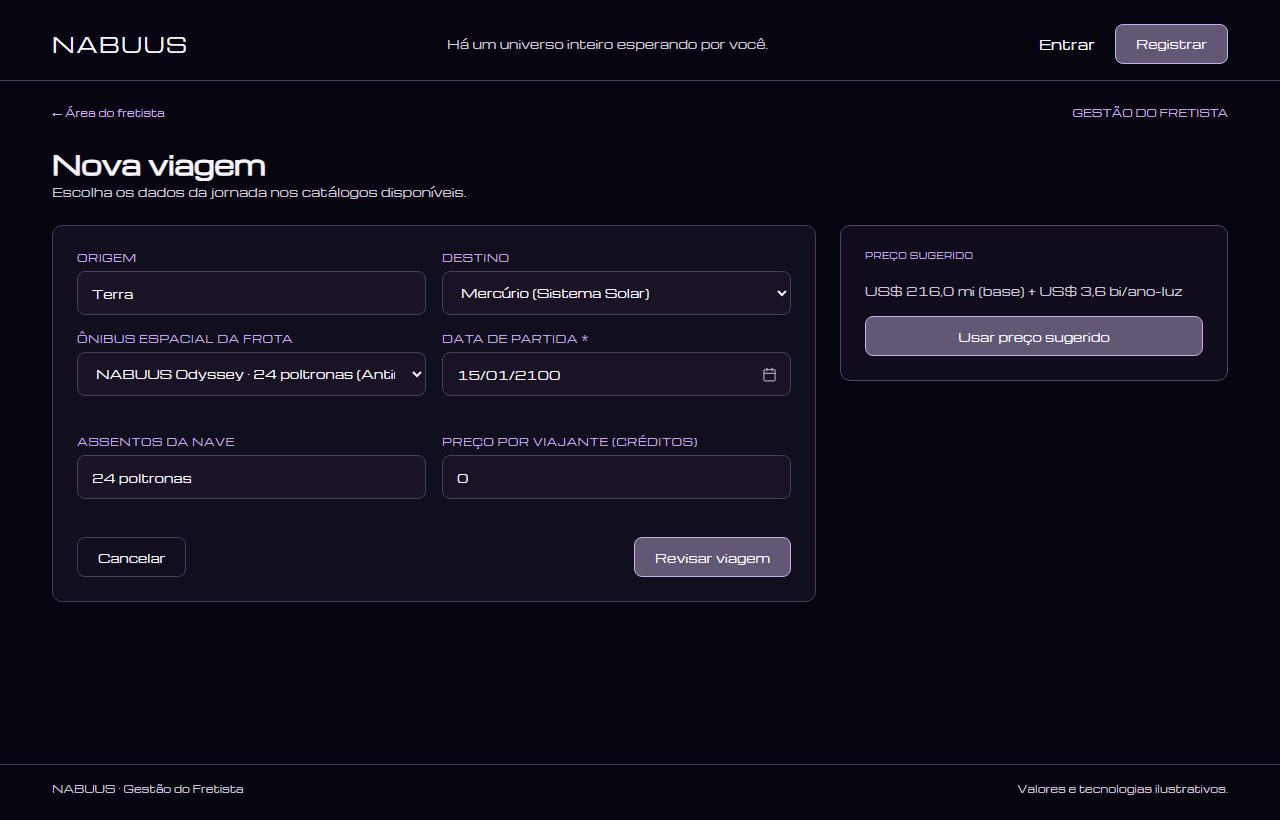
\includegraphics[width=0.86\textwidth, keepaspectratio]{figuras/tela-fretista.jpg}}
    \caption{Painel do Fretista --- Publicação de viagem com assentos vinculados à nave e preço sugerido dinâmico.}
    \label{fig:tela-fretista}
\end{figure}

\begin{figure}[H]
    \centering
    \fbox{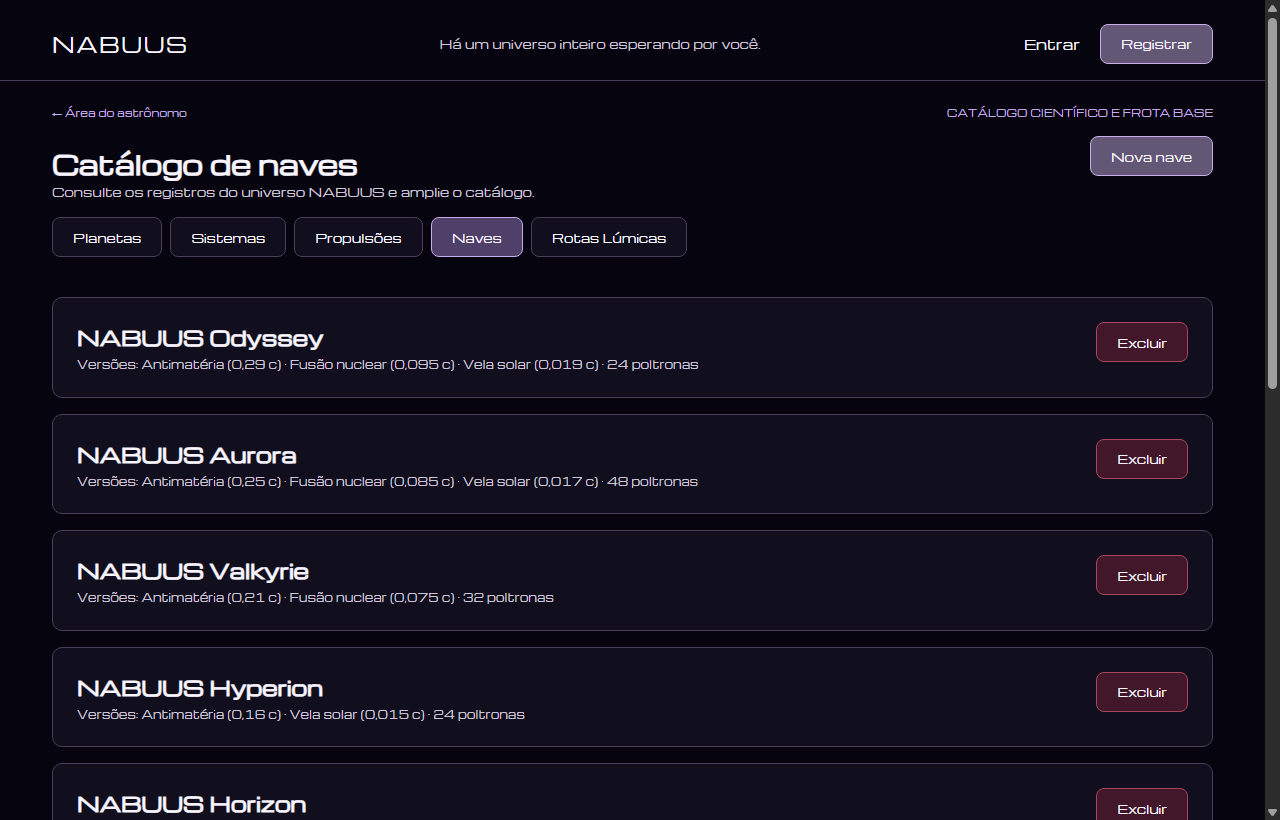
\includegraphics[width=0.86\textwidth, keepaspectratio]{figuras/tela-astronomo.jpg}}
    \caption{Painel do Astrônomo --- Catálogo técnico da frota (\texttt{24}, \texttt{32} ou \texttt{48} poltronas) e propulsões.}
    \label{fig:tela-astronomo}
\end{figure}

\end{document}
